\chapter{Introducere}
\section{Context}

Ministerul Educației Naționale (MEN) își propune cumpărarea manualelor școlare la un preț cât mai avantajos și cu o calitate cât mai bună \cite{minister}. Astfel, prin intermediul Centrului Național de Evaluare și Examinare (CNEE), Ministerul organizează anual licitații deschise pentru achiziționarea acestora. Pentru fiecare tip de manual (de exemplu, un manual de matematică pentru clasa a VI-a), Ministerul încheie contracte cu editurile pe o perioadă de 4 ani, după care sunt organizate noi licitații.

Evaluarea manualelor se bazează pe criterii tehnice, iar pentru ca un manual să fie declarat câștigător, acesta trebuie să obțină un punctaj de cel puțin 95 de puncte din 100. La un singur manual, pot câștiga mai multe edituri dacă această condiție este îndeplinită. Manualele trebuie să respecte un caiet de sarcini stabilit de MEN și CNEE. Astfel, câteva cerințe generale privind manualele digitale sunt: 
\begin{itemize}
	\item Accesarea manualului digital se face printr-un fișier de tip "index.html".
	\item Folderul director să nu depășească 600 MB.
	\item Paginile HTML să fie responsive (la o rezoluție de 1024x768 pixeli să nu apară bare de scroll orizontale).
	\item Manualul să poată fi utilizat pe fiecare browser din această listă: Google Chrome 31+, Mozilla Firefox 25+, Internet Explorer 10+, Safari 7+.
	\item Varianta digitală să cuprindă integral conținutul manualului din varianta tipărită.
\end{itemize}

Procesul de creare a unui manual tipărit și a unui manual digital se desfășoară conform următoarei diagrame:
\begin{figure}[H]
	\centering
	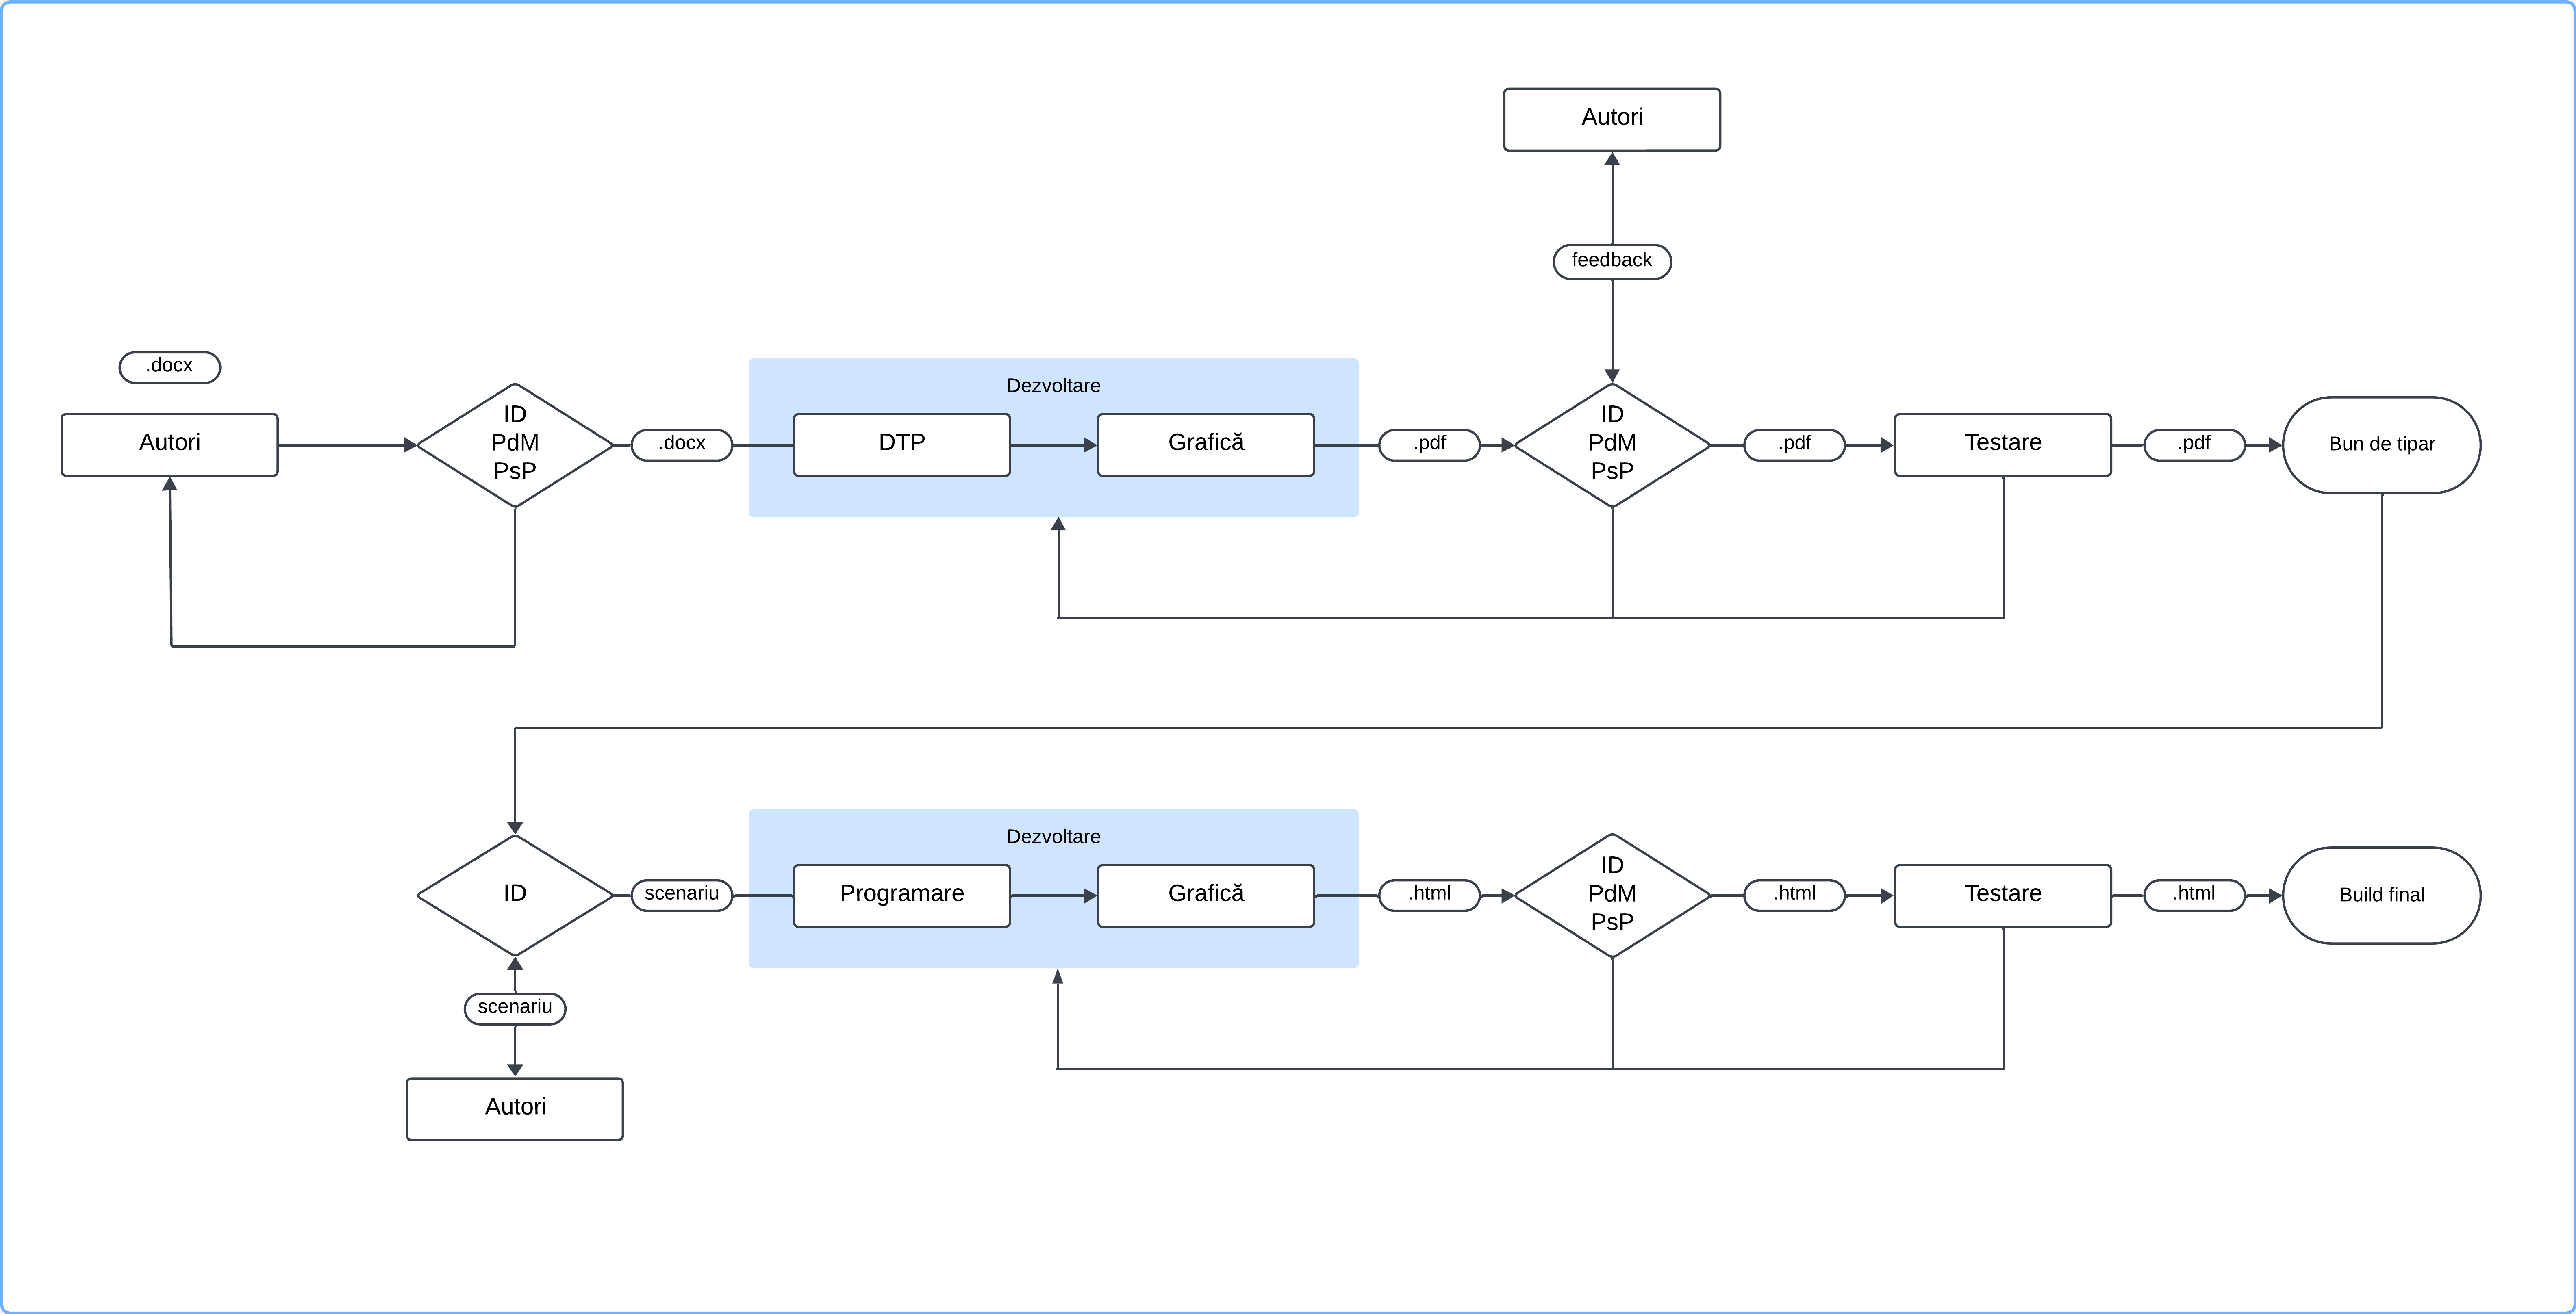
\includegraphics[scale=.3]{Figura1_1}
	\caption{Procesul de creare a manualelor tipărite și digitale}
	\label{fig:Figura1_1}
\end{figure}

\noindent
Legendă:
\begin{itemize}
	\item \textbf{ID} - Instructional Designer; persoana care pune în pagină conținutul și care creează un design pentru manual.
	\item \textbf{PdM} - Product Manager; persoana care supervizează tot procesul de creare.
	\item \textbf{PsP} - Psihopedagogic; persoana care propune modificări pentru conținut.
	\item \textbf{DTP} - Desktop Publishing; procesul prin care un manual este creat pentru a fi tipărit.
	\item \textbf{Grafică} - pasul în care se creează imaginile.
	\item \textbf{Programare} - procesul de a scrie cod HTML pentru conținutul dat de ID.
\end{itemize}

Procedura de creare pornește de la autori. Aceștia realizează un manuscris în format DOCX cu informațiile care vor apărea în manual. Ulterior, ID-ul, PdM-ul și PsP-ul verifică documentul și decid dacă sunt modificări de făcut. În momentul în care documentul este validat, procesul se împarte în două ramuri; o ramură pentru partea de tipar și alta pentru partea digitală.

Pentru dezvoltarea manualului de tipar, ID-ul structurează conținutul și toate detaliile care țin de punerea în pagină, iar după aceea echipa de grafică creează imagini. Tehnologiile folosite în acest proces sunt Adobe InDesign și Adobe Illustrator.

Adobe InDesign este o aplicație complexă de creare și structurare a documentelor, care poate să genereze documente cu rolul de a fi tipărite \cite{adobe2007adobe}. În cadrul realizării manualelor în format PDF, această aplicație este folosită pentru a pune în pagină informațiile date de autori într-un mod structurat și uniform.

Adobe Illustrator este un program de design grafic folosit pentru crearea de ilustrații, logo-uri sau chiar diagrame \cite{tupper2021}. În cazul manualelor, programul este folosit pentru a crea diferite imagini asociate cu textul, care îmbunătățesc aspectul vizual.

După acești pași, va rezulta o variantă inițială a manualului, exportată din Adobe InDesign în format PDF. Din acest punct se fac  verificări, atât pe partea de conținut dată de autori, cât și pe partea de redactare realizată de ID. Dacă nu există greșeli, se exportă manualul în versiunea lui finală. Dacă apar greșeli, se reiau pașii anteriori.

În diagrama de mai sus, la a doua parte de dezvoltare se sare peste pasul de grafică deoarece imaginile sunt obținute de la prima parte de dezvoltare, cea a manualului tipărit.

Manualul digital este creat într-un mod direct. După ce manualul este disponibil în format PDF, textul din acesta este extras și plasat într-un fișier HTML, împreună cu clasele și stilurile necesare. Deși este un proces simplu, acesta poate să dureze până la trei săptămâni pentru un manual de 200 de pagini. 


\section{Motivație}

În calitate de angajat al editurii Intuitext, am lucrat pe partea de conversie a manualelor în format digital și am observat cât de repetitiv este procesul și de cât de multă atenție este nevoie la detalii. Fiind un volum mare de manuale, riscul de a face greșeli era ridicat. În procesul de creare a manualului digital, orice greșeală reparată necesita retrimiterea manualului către echipa de testare până când toate erorile erau corectate. Acest lucru prelungea timpul în care un manual digital era finalizat.

Din dorința de a optimiza acest proces meticulos, am venit cu propunerea de a crea o aplicație care să automatizeze conversia.

Aplicația se folosește de datele pe care le extrage din manualul în format PDF: mărimea textului, fontul, culoarea textului, culoarea de fundal. Pe baza acestor date, aplicația recunoaște ce stiluri trebuie aplicate asupra textului și le scrie într-un fișier HTML. Fiecărei pagini din manualul tipărit i se asociază câte o pagină HTML.


\section{Scopul lucrării}

Scopul aplicației descrise în această lucrare este de a reduce timpul pe care angajații îl consumă pentru a converti manuale din format PDF în format HMTL. Beneficiul principal al acestei aplicații este creșterea profitabilității companiei într-un mod indirect. Timpul petrecut de angajați pentru transformarea manualelor va fi redirecționat către alte proiecte.

Un alt avantaj al aplicației este reducerea intervenției umane în procesul de transformare, ceea ce diminuează riscul apariției greșelilor. Acest lucru conduce la economisirea unui timp suplimentar deoarece nu trebuie să se reia pasul de testare de foarte multe ori.

În caietul de sarcini dat de MEN și CNEE este menționat faptul că tot conținutul din varianta de tipar a unui manual trebuie să apară și în varianta digitală, dar nu este nicio regulă care să precizeze că manualele trebuie să păstreze aceeași formatare.

Acest lucru ușurează procesul de automatizare deoarece permite schimbarea structurii unei pagini cât timp se păstrează ordinea logică a elementelor. De exemplu, unele pagini sunt împărțite în două coloane cu exerciții pe stânga și pe dreapta; nu este necesar să fie păstrată aceeași formatare atât timp cât se păstrează ordinea conținutului.


\section{Domenii abordate}

Domeniile abordate pentru realizarea aplicației sunt:
\begin{itemize}
	\item \textbf{Software development} - aplicația a fost dezvoltată folosind tehnici de bază, într-un mod simplu și eficient.
	\item \textbf{Automatizarea} - procesul de conversie a manualelor din format PDF în format HTML.
	\item \textbf{Natural Language Processing} - subdomeniu al inteligenței aritificiale, utilizat pentru a recunoaște structuri de text pe baza unor criterii.
\end{itemize}

 
\section{Obiective}

Pe parcursul dezvoltării aplicației, s-a ținut cont de următoarele aspecte:
\begin{itemize}
	\item \textbf{Similaritatea}: manualul digital generat să conțină într-o proporție cât mai mare elementele care sunt și în varianta tipărită.
	\item \textbf{Simplitatea}: structura codului HTML să fie organizată într-un mod cât mai ușor de modificat de alte persoane.
	\item \textbf{Viteza}: timpul de procesare să fie cât mai scurt.
	\item \textbf{Adaptabilitatea}: aplicația de automatizare să poată fi folosită pentru orice tip de manual, indiferent de materie sau de clasă.
\end{itemize}


\section{Structura lucrării}

Lucrarea este structurată în următoarele capitole:
\begin{itemize}
 	\item \textbf{Introducere}: prezintă scopul aplicației și aspectele care au fost luate în considerare la dezvoltarea acesteia.
 	\item \textbf{Soluții similare}: descrie soluțiile existente pe piață, le analizează și indică limitele sau inconvenientele lor.
 	\item \textbf{Tehnologii folosite}: detaliază tehnologiile alese pentru această aplicație și motivele pentru care au fost selectate.
 	\item \textbf{Soluție propusă}: este împărțită în patru subcapitole mai mici. Urmează cursul unui proces de automatizare: citirea, curățarea, gruparea și scrierea. 
	\item \textbf{Concluzii}: prezintă rezultatele aplicației și aspectele care pot fi îmbunătățite pe viitor. 
\end{itemize}

În subcapitolul de citire este descrisă metoda de extragere a informațiilor din documentul PDF, inclusiv extragerea imaginilor și procesul de obținere a culorii de fundal a textului.

În subcapitolul de curățare sunt identificate și șterse segmentele de text care nu vor apărea în varianta digitală.

În subcapitolul al treilea se prezintă metoda de grupare a textului în funcție de paragraful din care face parte.

În ultimul subcapitol se realizează procesul de scriere în fișierul HMTL și sunt identificate segmentele de text care nu au fost recunoscute de program și care vor fi introduse manual.
